\chapter{Introduction}
This chapter introduces automatic text summarization. Following section presents the background. Problem statement highlight the challenges to overcome.
Objectives of my research,  limitation and scope are described at the end of the chapter.
\section{Background}
Before formally defining automatic summarization let us look at what motivates the researchers from distinct disciplines to contribute to this field since 1960s.
In an IDC(International Data Corporation) white paper  ``The Expanding Digital Universe'' attempted to forecast the size of digital universe. One of the 
key findings stated that the amount of information created would surpass the storage capacity available for the first time in 2007.

\begin{figure}[!h]
\centering
\subfigure[predicted growth in digital universe by 2010 ]{
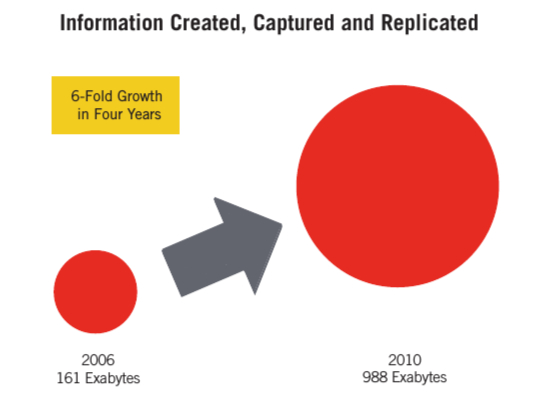
\includegraphics[scale=0.5]{infogrowth}
\label{fig:subfig1}
}
\subfigure[Information vs storage available]{
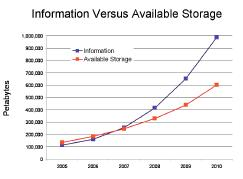
\includegraphics[scale=1]{fig2}
\label{fig:subfig2}
}
\caption{Expanding digital universe}
\end{figure}

The report predicted six fold growth by 2010 computing the size of the digital 
universe up to 988 exabyte(1 exabyte = 1000 petabytes, 1 petabyte = 1000 
terabytes) as depicted by figures 1.1 a and b.  

Initially Internet contained only static contents i.e. text that does not 
change over time, however with the passage of time Internet technologies 
facilitated its users
to socialize and share information via on line discussion and blogs both of 
them have also contributed in the expanding the Internet. According to 
wikipedia, 
\emph{Technorati} an Internet search engine for searching blogs, was indexing 
112.8 million pieces of tagged social media.
A chart from \emph{Technorati} is included to depict continuous weblogs growth. 
\begin{figure}[h]
 
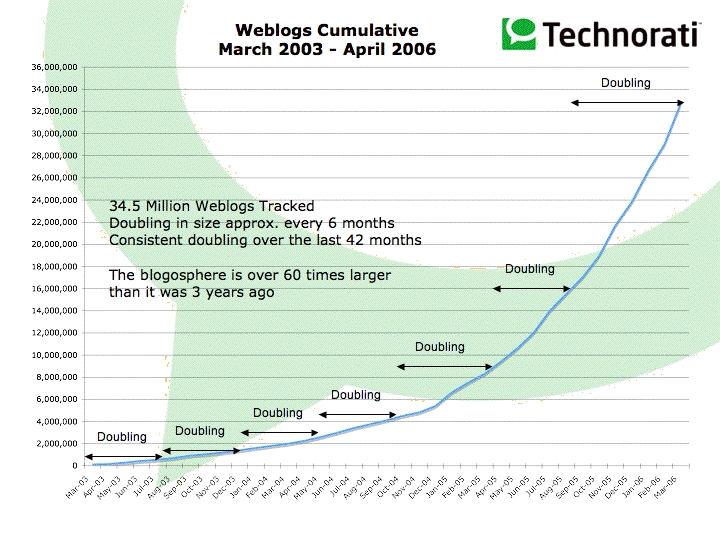
\includegraphics[width=0.9\textwidth]{blogosphere}
 \caption{\singlespace The blogo sphere is 60 times larger than it was 3 years 
ago}
\end{figure}

\begin{figure}[h]
 
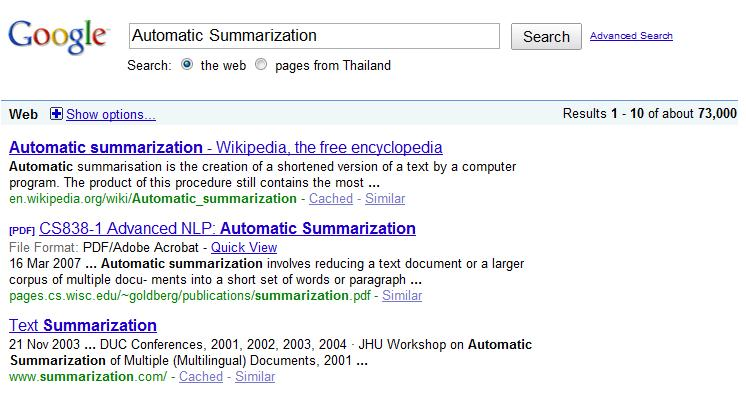
\includegraphics[width=0.9\textwidth]{googlesnapshot}
 \caption{\singlespace Indicative summary accompanies search results to aid 
user in selecting proper link}
\end{figure}
To address the difficulty of retrieving the desired information from such 
incredible volume of data(also termed as information overload) various tools 
and techniques were
developed. Search engines were developed to aid the user requesting for 
information. Search engines can not always accurately handover single best 
document as a result of 
a query rather provide a ranked list of document, the decision of selecting the 
best result is completed by the user.

The decision of the user is dependent on a useful text segment (the summary of 
the information that is associated with each result returned), without which 
it would be impossible to read bulk of full length documents and select what is 
required. 


Eduard Hovy in the book ``The Oxford handbook of computational linguistics'' 
defines summary as ``summary is a text that is produced from one or more texts, 
that contains a significant portion of the information in the original text(s),
and that is no longer than half of the original text(s).''

To better understand what a summary is, a short news article from CNN with its 
summary is included as an example:

\textbf{Sample document}

\textsf{England coach Fabio Capello has signed an amended contract that will 
keep him in charge of the national side until after the European Championships 
in 2012,
the Football Association (FA) has announced.}
\begin{figure}[h]
 

\includegraphics[width=0.9\textwidth]{mainstory}
 \caption{\singlespace Indicative summary accompanies search results to aid 
user in selecting proper link}
\end{figure}
\textsf{The new deal removes a break clause for both the FA and Capello, and 
comes after speculation that European
champions Inter Milan wanted the 63-year-old as their new boss to replace Jose 
Mourinho, who joined Real Madrid. The news came just hours before England's 
squad flew out to the World Cup finals in South Africa that begin on June 11. 
Capello added: ``I am very happy about this and would like to thank David 
Richards
[Club England chairman] and the FA for their continued support and assurances 
about my future.''
``I always wanted to stay until the end of my contract. In South Africa we are 
totally focused on the World Cup.''
Capello took charge of England in December 2007 and led them to top spot in 
their group during World Cup qualification.
Former FA chief executive David Triesman had been negotiating with Capello over 
his contract until he was forced to resign after claims made by a British 
newspaper.
Club England chairman David Richards quickly picked up the talks, leading to 
Wednesday's announcement.
Richards told the FA's Web site: ``We're very pleased to have Fabio's 
commitment for another two years and it's good that we have been able to 
resolve 
this before the team flies to South Africa.''
``Now we can all concentrate on the World Cup and give Fabio and the players 
our full support.''
England's first game at the World Cup is against the United States in 
Rustenburg on June 12.}

\textbf{Summary of sample document}

\textsf{The Football Association(FA) has announced that England coach Fabio 
Capello has signed an amended contract that will keep him in charge of the 
national side until after the European Championships in 2012.}

Summaries are mostly written by authors skilled in the art of vocabulary and 
composition. It would be ideal to obtain the summary of each and every document 
available 
on the Internet to help the users save time and cost but it is not possible. 
Summarization can however be semi or fully automated. Many systems and toolkits 
have been 
written to generate summary automatically. SUMMARIST a summarizer by Eduard 
Hovy and his team produces extract summaries in five different languages. Open 
text summarizer
is an open source tool for summarizing text. Classifier4J is a java API that 
has features for extracting text. Apache Lucene and opennlp tools are few other 
software 
libraries that contain essential components useful for developing summarization 
systems. 
\section{Problem Statement}
Summarizing essentially means understanding the source document in order to 
obtain core information the author intends to convey and then expressing the 
information 
completely in lesser words. The completeness and conciseness criteria are 
opposite in nature, trying to improve one will effect the other negatively, 
however it is difficult
for both a human evaluator and an automated system to measure informativeness 
of contents most evaluation mechanisms use length of document and its summary 
for evaluating 
the quality of summary. Understanding a document becomes difficult for two 
reasons, first a text document is not a database file where each piece of 
information is 
labeled and repeated with a regular pattern throughout the file, rather text 
documents like news articles, essays, reports, etc. are unstructured, where 
important 
information is scattered throughout the document without a regular pattern. 
Second reason is the nature of the words. A word can give different meanings 
depending on 
the context in which it is used. For example the word burn in the following 
sentences, `` How to easily burn 200 calories a day?'', and `` Please burn your 
thesis work on CDs and handover to the secretary''. Similarly different words 
can be used to convey same meanings. For example goal, target, objective can be 
used to convey
same message.
The reasons discussed above make the problem of generating a summary 
challenging.
Different approaches have been adopted by researchers from various discipline 
to summarize text. Statistical approach uses word frequency to determine key 
features of 
text, ignoring the structure of the document. Although this approach is very 
popular and frequently used in information retrieval, promising results are 
only possible for
huge corpus containing lengthy documents. Simple counts are not enough to 
determine all features of text and the semantics contained in it. Natural 
language processing(NLP) 
techniques have been developed to deal with the complexities of semantics. 
These techniques try to analyze text relying on domain knowledge. NLP remains 
computationally
expensive,and language dependent.
It also suffers from inherent text characteristics such as author's writing 
style. Many heuristics are commonly used by different summarizing systems.
Heuristics are also limited to the type of text. Since no single approach can 
tackle the task of analyzing and summarizing text comprehensively, techniques 
from two different
approaches are often used in combination.


\begin{figure}[h]
 
\includegraphics[width=0.9\textwidth]{textmargin}
 \caption{\singlespace Encapsulated text in left margin help to learn and revise 
important information quickly}
\end{figure}
As discussed in the previous section due to information overload, the user is 
forced to browse for information since accurate retrieval of the desired 
information
is not possible. Reducing the contents and representing the user with minimum 
possible words can be very useful. 
\section{Objectives}\label{ch1:obj}
The objective of my research study is to represent a document by as few words as 
possible. The core of my work is centered around the fact that most English 
sentences 
tend to convey information in three segments i.e. subject, verb and object. This 
idea of representing a given text into three chunks of text (possibly only 3 
words
 or more) is termed as \emph{text encapsulation}. This problem can be thought of 
as a  shorter version of text summarization problem. Text encapsulation can 
reduce a long 
 sentence to three basic components subject, verb and object which is the 
objective of my research. 
 Following tasks are part of my research objective:

\begin{enumerate}
 \item Extract important units(sentences) in a given text
 \item Determine frequent subunits(phrases) in the given text
 \item Parse extracted units containing frequent subunits for noun, verb, noun 
pattern.
\end{enumerate}

Following assumptions will be taken into account for the research project.
\begin{enumerate}
 \item Source document should be in English.
 \item Single document is used as source. 
 \item Summary may contain discrete phrases.
 \item Sentences generated convey approximate meanings.
\end{enumerate}

For example here is the encapsulation for the news article in previous section:\\
\textbf{Encapsulation of example news article}

\textsf{England coach Fabio Capello signed an amended contract, will keep him in charge until European Championships 2012.}

Encapsulated text is not only useful for time-effective learning, it is very handy for readers who have come back for revision after long time. This technique is frequently used by publishers, for publishing books
on newer version of software tools, so that experts can quickly scan encapsulation in the margins and focus on new features introduced. Figure 1.4  is an example
of text encapsulation.




% \section{Thesis Outline}  
% 
% \begin{description}
%  \item {Chapter 2} presents research literature. Important and recent contributions are cited.
%  %\item {Chapter 3} elaborates the fundamentals of summarization systems.
%  \item {Chapter 3} contains the methodology. 
%  %\item {Chapter 5} 
% 
% \end{description}


\clearpage 
